\chapter{使用 \headinglatin{\ksonline}}\label{ch:online}
\index{Zaixian ban@線上版}

\ksonline{} 將工具箱工作區放在瀏覽器中，無須在本機安裝客戶端。結構編輯、工作流與結果分析仍在主視窗中進行，實際運算由伺服器完成。瀚海量子\regmark{}官方線上版即將推出，並支援叢集私有化部署。透過所選部署提供的入口登入賬號後，便可進入分配的工作空間。

線上版與桌面應用最需要區分的地方是檔案和會話。本機檔案需要上傳，專案通常儲存在雲端“檔案”面板中，下載後才得到個人計算機上的副本。關閉網頁、返回入口和登出也有不同含義。本章透過一個矽結構專案，把這些操作串成一次完整的練習。

\section{進入自己的工作空間}

\subsection{開始前準備什麼}

準備好所選部署提供的線上地址、可用賬號，以及隨書的小型結構檔案。首次註冊可能需要邀請碼，按部署頁面給出的註冊方式操作。瀏覽器應能正常執行 WebGL，以便顯示三維原子結構。

儘量使用較大的瀏覽器視窗。視窗較小時，中央檢視與引數編輯區會同時變窄，長表單可能需要滾動。在筆記本上可以先收起暫時不用的側邊面板；這樣仍能保留工具欄和正在編輯的文件。

同一個工作空間使用一個活動瀏覽器標籤頁。若已在另一標籤頁開啟工作區，可返回該標籤頁繼續使用，或關閉舊連線後重新連線。

\subsection{註冊賬號}

固定入口首先顯示登入頁。需要新賬號時，切換到註冊頁，按表單依次填寫。賬號名使用小寫字母、數字或連字元，以字母開頭，長度為 3--32 個字元；密碼長度為 12--128 個字元，並需再次輸入確認。

註冊還需要備忘問題、備忘答案和邀請碼。問題和答案用於找回密碼，應便於自己記憶，並避免透露密碼。問題和答案填寫後，點選 \ui{註冊賬號}，成功後返回登入頁。


\subsection{登入並等待啟動}

\begin{steps}
\item 在固定入口的登入頁填寫個人賬號資訊。
\item 點選 \ui{登入並開啟工作空間}。
\item 等待入口顯示工作空間準備狀態。第一次啟動可能比以後更久。
\item 工作空間就緒後進入工具箱主介面；如果入口顯示 \ui{開啟工作空間}，點選該按鈕繼續。
\item 確認上方出現工具欄，左側可開啟\ui{專案瀏覽器}和\ui{檔案}面板，中央文件區能夠響應操作。
\end{steps}

入口可能顯示“正在啟動”“已就緒”等狀態。狀態變化時保持頁面開啟即可，無需連續點選啟動。若單位的併發名額暫時已滿，按入口提示稍後重試；是否可增加名額由部署方決定。

\section{認識線上版中的檔案}
\index{Yunduan wenjian@雲端檔案}

\subsection{專案樹與檔案樹}

左側專案瀏覽器與檔案面板透過側邊按鈕分別檢視。同一時刻顯示其中一個；需要從雲端目錄回到結構時，點選專案瀏覽器的側邊按鈕，需要檢查上傳檔案時，再切迴檔案面板。

專案瀏覽器組織當前專案內部的內容，例如結構、工作流、計算資料和圖形。左側 \ui{檔案} 面板則顯示雲端目錄中的檔案和資料夾。一個 \file{.ks} 檔案可以包含許多專案項，因此兩棵樹顯示的內容不會相同。

把專案理解為一本裝著實驗材料與結果的記錄本，雲端資料夾就是存放記錄本的書架。匯入結構是在記錄本中增加材料；儲存專案則把當前記錄寫入一個 \file{.ks} 檔案。只上傳一個 CIF 檔案，相當於把原始材料放上書架，還沒有把它放入當前記錄本。

\begin{table}[htbp]
\centering
\caption{常見操作的結果}
\begin{tabularx}{\linewidth}{lX}
\toprule
操作 & 結果 \\
\midrule
上傳 & 將本機檔案複製到當前雲端目錄。\\
匯入 & 讀取檔案內容，在當前專案中增加結構或工作流等物件。\\
儲存 & 將當前專案寫入雲端的 \file{.ks} 檔案。\\
下載 & 將選中的雲端檔案另存到自己的計算機。\\
開啟專案 & 讀取一個 \file{.ks} 檔案作為當前專案。\\
\bottomrule
\end{tabularx}
\end{table}

\subsection{檔案面板的日常操作}

檔案樹按名稱排列，資料夾排在檔案前面。展開資料夾可以檢視下一層內容；表頭箭頭切換名稱升序和降序。右側 \ui{⋮} 開啟檔案操作選單，也可以在條目上右擊。

選中資料夾後，面板底部顯示所在目錄；選中檔案後還會顯示檔案大小。上傳、新建資料夾和首次儲存專案會使用當前目錄，因此進行這些操作前，先看一眼底部路徑。

\ui{重新整理} 重新讀取目錄，通常保留已展開的資料夾與選中項。若在其他操作後暫時看不到新檔案，可以先重新整理，再檢查自己是否展開了正確的資料夾。目錄中的檔案數量很多時，按課題和練習分資料夾，比反覆在長列表中查詢更方便。

圖\ref{fig:online-workspace-silicon}給出本例儲存後的工作區，左側顯示檔案面板。需要檢視專案內的結構和工作流時，點選專案瀏覽器的側邊按鈕。

\section{練習：建立矽結構專案}

\subsection{建立練習目錄}

本例使用隨書的 \file{examples/silicon.cif}。也可以換用其他小型結構，檔案操作步驟相同。為了清楚區分原始結構、工作專案和下載副本，先為本次練習建立獨立目錄。

\begin{steps}
\item 在 \ui{檔案} 面板選中根目錄或選定的工作目錄。
\item 開啟 \ui{⋮ → 新建資料夾}，輸入 \file{Si-study}。
\item 確認檔案樹中出現新目錄，選中並展開它。
\item 檢查面板底部路徑，確認當前目標是 \file{Si-study}。
\end{steps}

\subsection{上傳結構檔案}
\index{Shangchuan@上傳檔案}

\begin{steps}
\item 在 \file{Si-study} 目錄中開啟 \ui{上傳}。
\item 在瀏覽器或系統檔案選擇器中選中本機的矽結構 CIF。
\item 確認選擇，等待上傳進度完成。
\item 回到檔案樹，核對檔名與大小，必要時點選 \ui{重新整理}。
\end{steps}

支援原生檔案選擇器的瀏覽器會直接顯示系統視窗；其他瀏覽器可能先顯示頁內選擇按鈕，再由按鈕開啟檔案視窗。兩者都從自己的計算機選擇檔案。選完後，在傳輸完成前保持頁面和傳輸視窗開啟。

檔案出現在雲端目錄中後，上傳即已完成。隨後將它匯入專案，才能在專案瀏覽器中檢視結構。

檔案上傳與匯入後的工作區見圖\ref{fig:online-workspace-silicon}。

\subsection{把檔案匯入專案}
\index{Daoru@匯入結構}

\begin{steps}
\item 在 \ui{檔案} 面板雙擊剛上傳的 CIF；也可以選中該檔案後選擇 \ui{匯入}。
\item 檢視專案瀏覽器，確認增加了結構項。
\item 檢視中央文件區，確認原子與晶胞已經顯示。
\item 拖動三維檢視觀察結構，用滾輪縮放，使晶胞完整地位於檢視內。
\end{steps}

現在，雲端 CIF 是原始檔案，專案中的結構則是後續建模和計算使用的物件。對專案結構做超胞、刪除原子或其他編輯，不會自動把原始 CIF 變成修改後的結構。需要保留整個工作過程時儲存專案；需要另一個結構檔案時使用相應匯出操作。

檔案樹中的 \file{.ks} 和 \file{.wf} 含義不同：雙擊 \file{.ks} 開啟專案，雙擊 \file{.wf} 匯入工作流。其他能識別的結構檔案按結構匯入處理。資料夾雙擊用於展開，不會匯入為結構。

\subsection{首次儲存專案}
\index{Baocun xiangmu@儲存專案}

\begin{steps}
\item 在 \ui{檔案} 面板確認選中 \file{Si-study} 資料夾。
\item 點選工具欄 \ui{儲存}，或使用 Ctrl+S；macOS 使用 Command+S。
\item 在頁內視窗輸入 \file{Si-ground-state.ks}，確認儲存。
\item 檢查檔案樹，確認該專案檔案出現在練習目錄中。
\item 檢視標題和儲存狀態，確認本次修改已儲存。
\end{steps}

\begin{figure}[!htb]
\centering
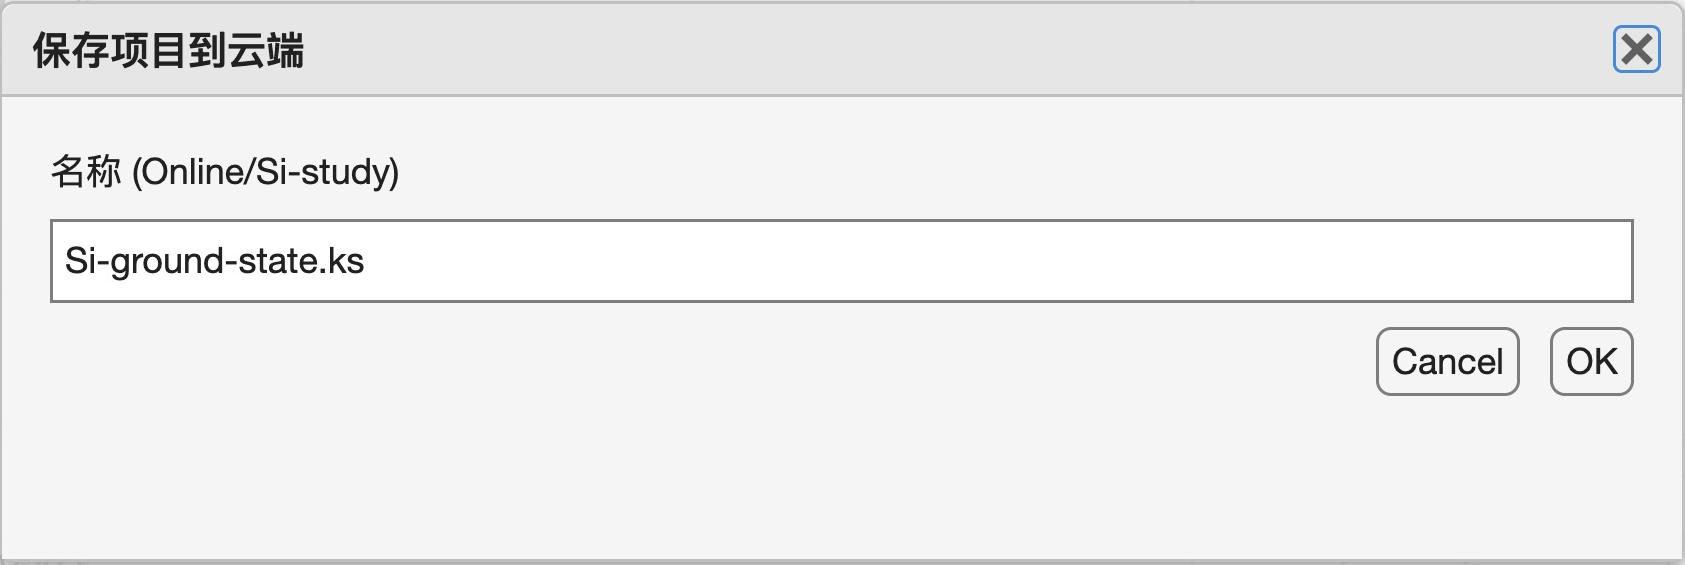
\includegraphics[width=\linewidth]{publication-assets/crop-5eed673aca0b27c69288.png}
\caption{儲存專案到雲端的名稱視窗。名稱欄填寫Si-ground-state.ks，括號內顯示當前選中的\file{Online/Si-study}目錄。}
\label{fig:online-save-project}
\end{figure}

檔名只填寫名稱，不需要輸入伺服器完整路徑。儲存視窗會使用所選目錄；沒有填寫 \file{.ks} 副檔名時，應用會補上。以後再次點選 \ui{儲存}，更新的是這個專案檔案。

若已經儲存過專案，在檔案樹另選資料夾後直接儲存，專案仍寫回原來的位置。想要改名、保留階段版本或放到另一目錄時，應使用 \ui{另存為…}。檔案面板選單中的 \ui{儲存專案到雲端} 也會詢問檔名，可用來把當前專案另存到所選目錄。

\begin{figure}[!htb]
\centering
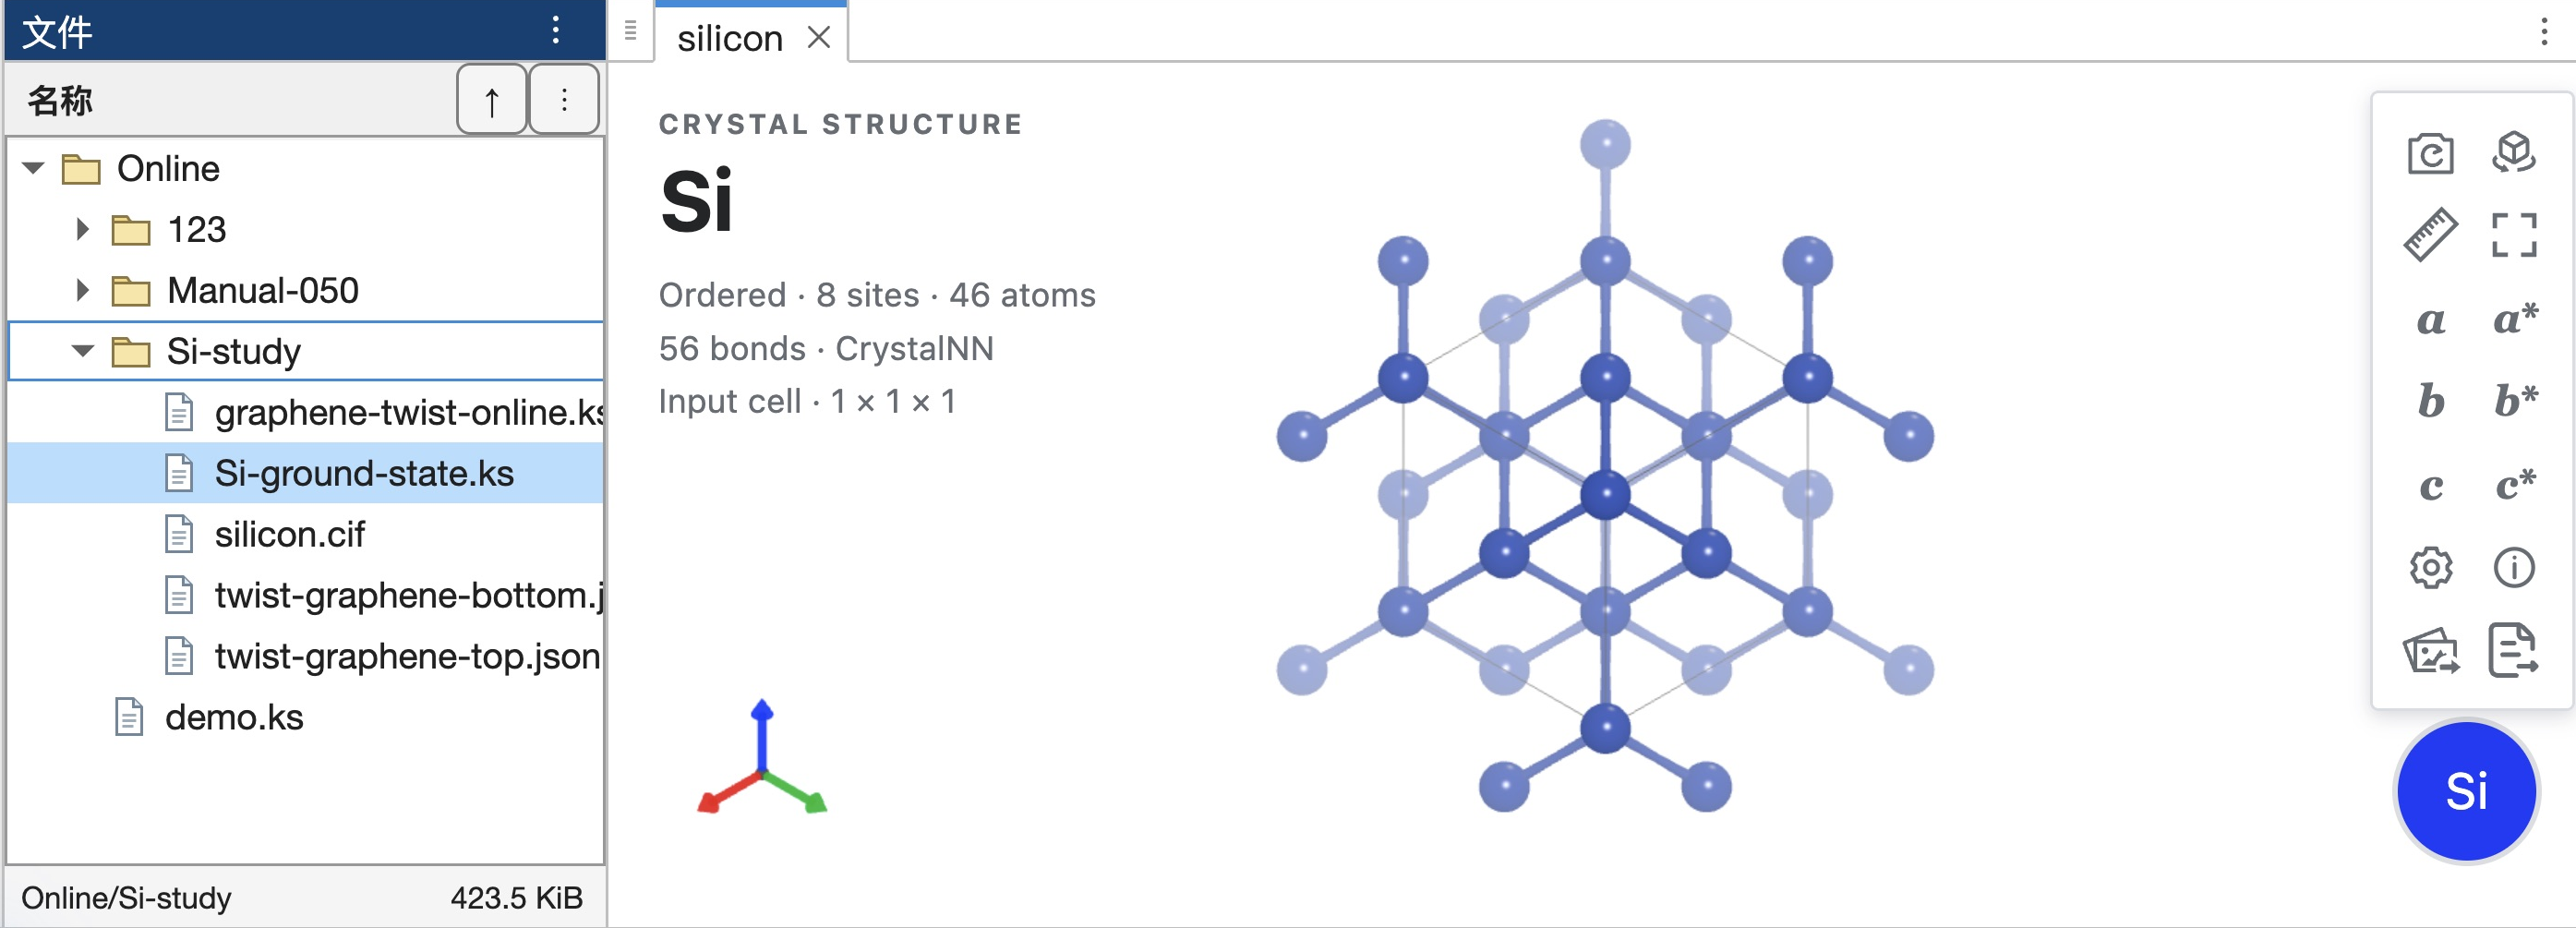
\includegraphics[width=\linewidth]{publication-assets/crop-11fbbbc4e8e9d6f1929d.png}
\caption{檔案與模型的佈局概覽。左側Si-study目錄中選中Si-ground-state.ks，中央顯示8個獨立位點及包含週期映像的46個顯示原子。}
\label{fig:online-workspace-silicon}
\end{figure}

圖\ref{fig:online-workspace-silicon}顯示檔案與模型的對應關係。8 sites用於核對模型位點數，46 atoms則包含週期映像。本節專案儲存矽結構，基態計算見第\ref{ch:workflows}章。

\subsection{另存一份用於比較的專案}
\index{Lingcunwei@另存為}

材料建模常需要比較不同超胞、缺陷或引數。在較大修改前儲存一份階段專案，可以讓後續比較更清楚。這裡先練習另存，不改變模型。

\begin{steps}
\item 在 \ui{檔案} 面板選中要放置副本的目錄。
\item 開啟儲存選單，選擇 \ui{另存為…}。
\item 輸入新名稱，例如 \file{Si-comparison.ks}。
\item 儲存後，檢查新檔案已經出現，原檔案仍然保留。
\end{steps}

另存後繼續編輯的是新專案檔案。給檔案命名時可以標明材料、處理和階段，例如“矽原胞”“矽超胞”“幾何最佳化後”；不必把所有計算引數都塞進檔名，詳細設定會留在專案中。

\section{將專案帶回自己的計算機}
\index{Xiazai xiangmu@下載專案}

\subsection{下載雲端檔案}

雲端儲存便於下次登入繼續工作；本機下載便於備份或與他人共享。二者可以同時使用。下載的是檔案當前已經儲存的內容，因此先儲存，再下載。

\begin{steps}
\item 選中 \file{Si-ground-state.ks} 或剛另存的專案。
\item 從右鍵選單或 \ui{⋮} 選擇 \ui{下載}。
\item 等待檔案準備完成。Chrome可能直接彈出本機儲存視窗；選擇資料夾、核對專案名後點選\ui{儲存}。
\item 沒有自動彈出本機視窗時，可使用頁內視窗提供的\ui{Save as…}；也可以點選\mbox{\ui{Browser download}}，用瀏覽器的原生下載方式儲存。
\item 等待瀏覽器下載列表顯示完成；若傳輸視窗另有\ui{Finish}，確認本機檔案已儲存後再點選。
\item 在自己的檔案管理器中核對專案名稱和檔案大小。
\end{steps}

\begin{figure}[H]
\centering
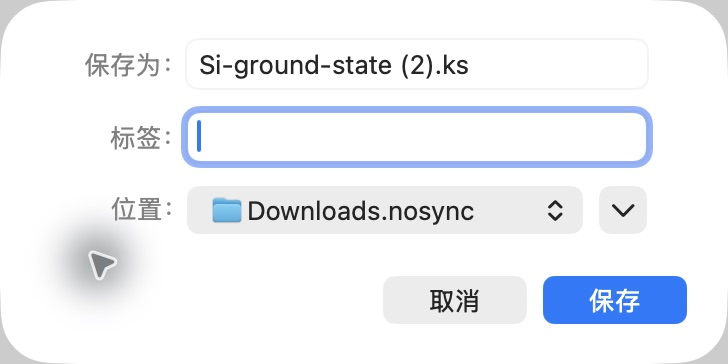
\includegraphics[width=72mm]{publication-assets/crop-348b0d07fb6f4cdab9d3.png}
\caption{macOS本機儲存視窗，以隨書矽專案為例。選擇資料夾並核對專案名後點選儲存；已有同名檔案時，瀏覽器可能在名稱後加上編號。}
\label{fig:online-project-download}
\end{figure}

瀏覽器設定可能讓檔案直接進入“下載”目錄，也可能每次詢問儲存位置。若不知道檔案去了哪裡，可以開啟瀏覽器下載列表檢視。若頁內視窗顯示\ui{Ready to download}，表示檔案已準備好交給瀏覽器；隨後仍需完成\ui{Save as…}、\mbox{\ui{Browser download}}或下載連結對應的本機儲存。本機儲存後，頁內準備視窗可能隨之關閉。應以瀏覽器的完成狀態和本機檔案為檢查點。

如果準備檔案失敗，視窗可能提供 \ui{Retry download}。點選後重新準備即可。取消下載不會取消雲端已經完成的儲存；想稍後下載時，可以重新在檔案樹選擇同一檔案。

\subsection{上傳下載的大小限制}

單個上傳或下載檔案最多為 128~MiB；一次上傳的檔案總計不超過 128~MiB，最多選擇 100 個。這個限制針對瀏覽器檔案傳輸，並不等於賬號的全部儲存容量。

隨著計算結果增加，專案可能明顯變大。下載前可以在檔案面板檢視檔案大小。超過傳輸上限時，使用部署方提供的大檔案傳輸方式。

本節儲存並下載的結構專案隨書提供為\file{examples/Si-ground-state.ks}，可用於核對矽結構和線上版檔案往返操作。

\section{檢視當前賬號}

連線賬號服務的線上版在主視窗上方顯示賬號名。開啟賬號名選單，選擇\ui{我的賬號}，可進入設定中的賬號頁；也可以從\ui{主頁 → 設定}進入該頁。賬號頁顯示當前賬號名、連線狀態和部署方給出的空閒釋放時長。

\begin{steps}
\item 確認上方顯示的是自己的賬號名，開啟\ui{我的賬號}。
\item 檢視連線狀態；綠色圓點與已連線文字用於識別當前會話。空閒時長表示無互動操作時保留會話的時間。
\item 若連線需要恢復，使用賬號頁的\ui{重新連線}，返回工作區後檢查專案與檔案。
\item 結束使用前先儲存專案；需要退出賬號時，再使用\ui{登出}。
\end{steps}

部署未提供賬號頁時，可從入口頁連線工作區。


\section{離開工作空間}

\subsection{臨時返回入口}

賬號選單中的 \ui{退出 KSSOLV Toolbox} 會返回入口，工作空間繼續保留至空閒超時。保留當前瀏覽器標籤頁時，入口中的 \ui{重連工作空間} 可以回到原介面，適合暫時檢視入口狀態後繼續工作。

這一操作與登出不同。暫時返回入口並不會立即釋放計算資源，也不會把專案自動儲存到磁碟。重要修改仍應先儲存。

完成第\ref{ch:first}章的氫分子計算後，可以用儲存的專案練習返回與重連：
\begin{steps}
\item 儲存當前專案，確認計算已經結束。
\item 開啟上方賬號選單，選擇\ui{退出 KSSOLV Toolbox}。閱讀保留工作空間的提示，確認後返回入口。
\item 核對入口顯示\ui{已返回入口，工作空間仍在執行}，再點選\ui{重連工作空間}。
\item 回到工作區後檢查原專案：SCF流程仍有Configuration、SCF與Plot三個節點，Results中的Run SCF資料集和EnergyConvergence曲線仍在。開啟曲線，確認可以繼續閱讀結果。
\end{steps}

\begin{figure}[!htb]
\centering

\includegraphics[width=122mm]{publication-assets/crop-432edbee8ecb03b7c537.png}
\caption{返回入口後的狀態與\ui{重連工作空間}按鈕。重連可回到原專案；\ui{登出並釋放例項}會結束工作空間。}
\label{fig:online-reconnect}
\end{figure}

\subsection{關閉或重新整理網頁}
\index{Chonglian@重新連線}

關閉網頁不等於登出。重新訪問同一固定入口時，如果原工作空間仍然存活，可以重新連線，並重新建立瀏覽器介面。專案、已開啟的結構與工作流等內容可以在同一執行例項中恢復；但臨時對話方塊、撤銷歷史和完整佈局不必然保持原樣。

重新整理頁面會重建瀏覽器介面。網路短暫中斷時，可等待連線恢復，或從固定入口重連；臨時離開時，可用賬號選單返回入口，再透過重連繼續工作。

\subsection{登出並釋放工作空間}

結束今天的工作，尤其是在共享計算機上，先儲存專案，再從賬號選單選擇 \ui{登出}，或在入口點選 \ui{登出並釋放例項}。確認後會結束訪問會話並釋放執行例項。

下一次登入會使用同一賬號的雲端檔案。此前儲存的專案和設定仍然保留，但僅在記憶體中的變數、未儲存修改和執行中的計算不能依靠登出後恢復。離開前先儲存專案，需要本機副本時再下載檔案。


\subsection{理解空閒釋放}

線上版的空閒釋放時間由平臺設定，當前值可以在賬號設定或入口提示中檢視。不同部署可能採用不同的時長，接近釋放時頁面會顯示提醒。鍵盤、點選、觸控和滾動表示存在互動操作；僅將標籤頁留在前臺，或讓狀態自動重新整理，並不延長空閒時間。

計算正在執行也不表示始終存在互動操作。安排較長任務前，應瞭解平臺對空閒釋放和長時計算的安排。需要使用獨立叢集佇列時，按照所用叢集的使用說明操作；完整 MATLAB\regmark{} 工具箱的遠端提交見第~\ref{ch:remote}~章。

\Needspace{6\baselineskip}
\begin{notebox}{再次登入後繼續工作}
再次登入後，在“檔案”面板找到練習目錄，雙擊已儲存的 \file{.ks}，即可繼續編輯結構、配置工作流或檢視結果。
\end{notebox}

\section{處理工作空間連線}

工作區底部的資源狀態用於瞭解當前執行環境的 CPU 和記憶體佔用。在按賬號分配資源的部署中，它反映分配給當前工作區的資源；普通容器部署也可能顯示宿主機環境。可結合狀態列標識與部署說明了解當前資源範圍。

工作流的資源選項取決於節點任務、求解方法和部署所支援的計算環境。配置時先選中目標節點，再檢視其資源面板；具體選擇與檢查方法見第\ref{sec:node-resources}節。主頁的\ui{並行}按鈕不代替節點資源設定，伺服器是否具備程序池或GPU支援也需按部署條件確認。

熟悉檔案操作後，可以繼續第~\ref{ch:first}~章的氫分子計算。先把隨書\file{h2.cif}上傳到自己的雲端目錄，再匯入當前專案。隨後建立SCF工作流，按該章填寫結構輸入和求解引數。

圖\ref{fig:online-h2-config}展示氫分子教程的結構輸入設定。選中節點後，使用\ui{工作流 → 配置節點}，向下檢視\ui{選項}。本例的結構配置節點標為\ui{Configuration}，對應\ui{Build Molecule}任務；選擇Molecule、結構h2、PBE、default贗勢、20 Ha、0 K與Nspin=1。SCF節點的求解方法和最大步數仍按第~\ref{ch:first}~章設定。

\begin{figure}[!htb]
\centering
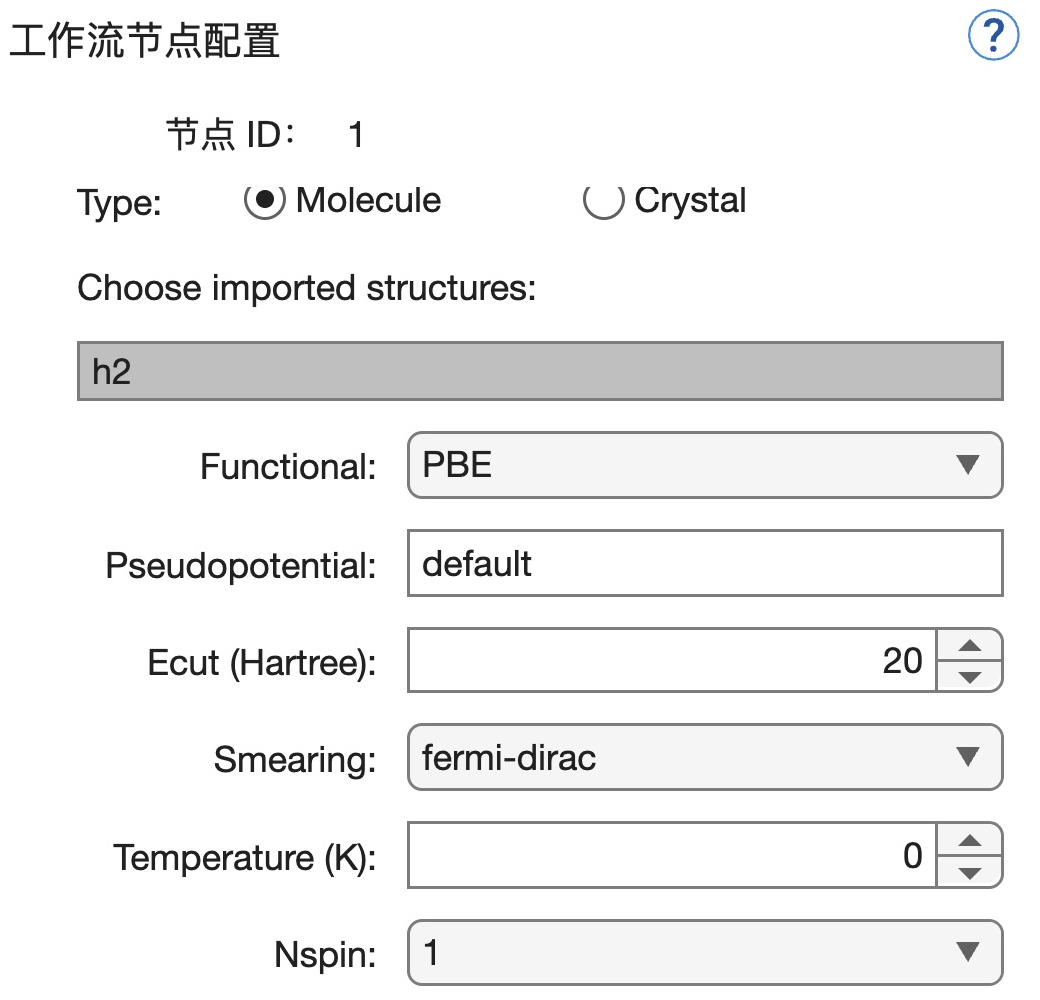
\includegraphics[width=88mm]{publication-assets/crop-434fe0ac4d3f46cfaf46.png}
\caption{氫分子工作流的結構輸入選項。所選h2結構和計算條件都在右側配置編輯器中核對。}
\label{fig:online-h2-config}
\end{figure}

參考計算在7步達到收斂，日誌與數值結果見第~\ref{ch:first}~章。計算結束後，點選專案瀏覽器側邊按鈕，展開\ui{Results}：\ui{Datasets}下的\ui{Run SCF}儲存這次執行的資料，\ui{Plots}下的\ui{EnergyConvergence}開啟收斂圖。

檢查日誌和曲線後，再次儲存專案，關閉當前專案，然後從\ui{檔案}面板雙擊儲存的\file{.ks}重新開啟。圖\ref{fig:online-h2-results}展示重新開啟專案後的結果分類，資料集與曲線分別儲存在對應分組中。再次雙擊\ui{EnergyConvergence}，可以讀到剛才七次迭代的收斂圖。最後從雲端下載專案，保留本機副本。

\begin{figure}[!htb]
\centering
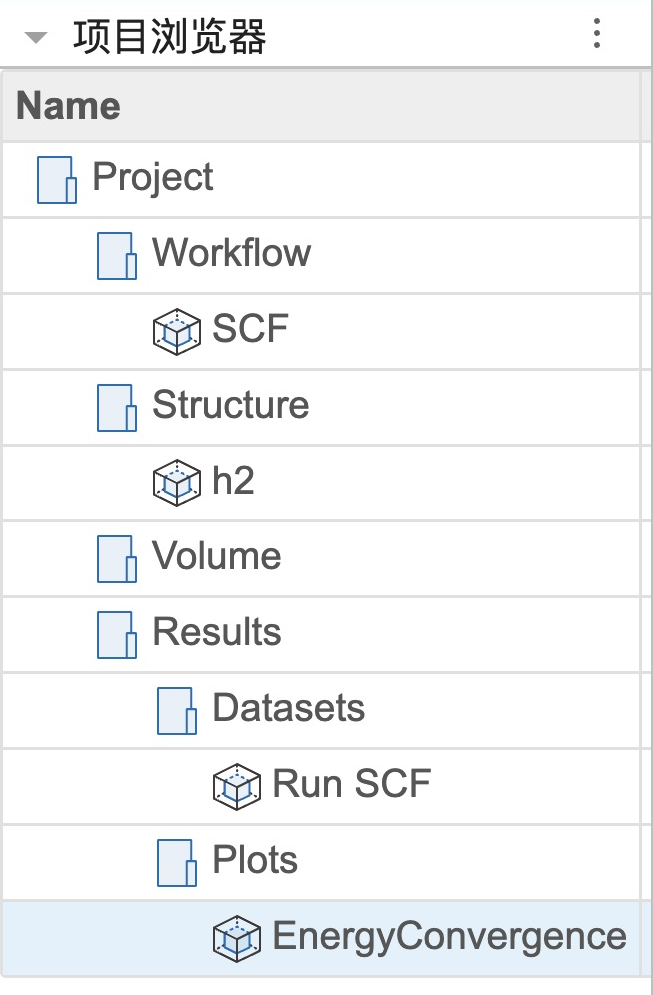
\includegraphics[width=55mm]{publication-assets/crop-c36a9eee3be02622a4d7.png}
\caption{氫分子專案的結果分類。Results包含Run SCF資料集與EnergyConvergence收斂圖；雙擊曲線條目可檢視迭代結果。}
\label{fig:online-h2-results}
\end{figure}

這樣，結構準備、伺服器計算、儲存與重新開啟就連成了一次完整練習。

連線失敗時先回固定入口，檢視工作空間是否仍在啟動。如果入口顯示 \ui{重試連線}，先使用此操作。持續不可用時，入口可能提供 \ui{重啟工作空間}；重啟保留已儲存檔案和設定，但結束當前記憶體會話，確認後再操作。

忘記密碼時，在登入頁點選 \ui{忘記密碼}，先取得個人備忘問題，再填寫答案和新密碼。重置過程會結束已有會話，成功後重新登入；若沒有設定問題或忘記答案，請聯絡管理員。

介面若提示“當前部署未啟用持久化檔案”，開啟檔案需從本機上傳，儲存時透過瀏覽器下載。離開前確認本機已有副本。
